\section{Learning Deep NBNN Representations for Robust Place
Categorization}\label{header-n666}

\emph{IEEE ROBOTICS AND AUTOMATION LETTERS, VOL. 2, NO. 3, JULY 2017}
{[}17{]}

\subsection{Introduction}\label{header-n668}

An important aspect of human-robot interaction is the ability of
artificial agents to understand the way humans think and talk about
abstract spatial concepts. To do this, an autonomous agent has to
extract information from its sensor to assign a semantic labels to a
specific place. In particular, this work focuses on assign label to
images. The most important challenges in identifying places come from
the complexity of the concepts to be recognized and from the variability
of the conditions in which the images are captured. In fact, scenes from
the same category may differ significantly, while images corresponding
to different places may look similar. The historical take on these
issues has been to model the visual appearance of scenes considering a
large variety of (shallow) learning models (e.g. SVMs, Random Forests),
but approaches based on learning deep representations have become
mainstream. Some work, like {[}19{]}, demonstrated the benefits derived
from feature extraction through convolutional deep neural networks.
Subsequent studies demonstrated the benefits of region-based approaches
(i.e. considering only specific image parts) in combination with
descriptors derived from CNNs, such as to obtain models that are robust
to viewpoint changes and occlusions. Other successful works tried to
bring back the notion of localities into deep networks, e.g. by
designing appropriate pooling strategies or by casting the problem
within the Image-2-Class (I2C) recognition statements, with a high
degree of success. Despite this, these methods implement the CNN feature
extraction and the classifier learning as two separate modules. This
leads to two drawbacks: first, choosing heuristically the relevant
localities means concretely cropping parts of the images before feeding
them to the chosen features extractor. Second, it would be desirable to
fully exploit the power of deep networks by directly learning the best
representations for the task at hand, rather than re-use architectures
trained on general-purpose databases like ImageNet. This work proposes
an approach for semantic place categorization which exploits local
representations within a deep learning framework. The method is inspired
by the recent work {[}18{]}, which demonstrates that, by dividing images
into regions and representing them with CNN-based features,
state-of-the-art scene recognition accuracy can be achieved by
exploiting an I2C approach, namely a parametric extension of the Naıve
Bayes Nearest Neighbor (NBNN) model. The deep architecture for semantic
scene classification seamlessly integrates the NBNN and CNN frameworks.
We automatize the multi-scale patch extraction process by adopting a
fully-convolutional network, guaranteeing a significant advantage in
terms of computational cost over two-steps methods. This is the first
attempt to fully unify NBNN and CNN, building a network in which the
NBNN error is back-propagated to the CNN in a unified end-to-end
training.

\begin{figure}[h!]
\centering
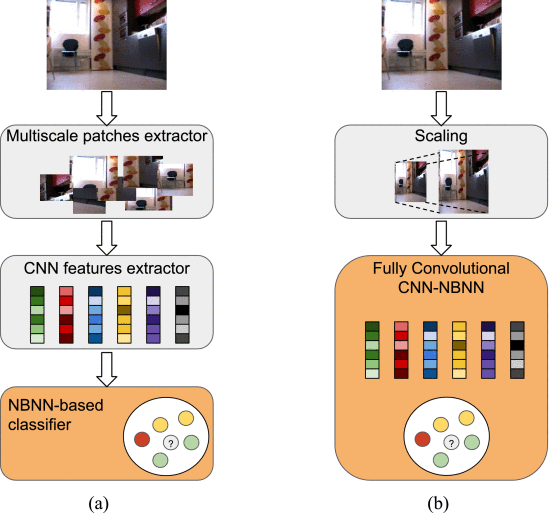
\includegraphics[width=0.6\linewidth]{images/NBNNdiff.png}
\caption{The standard NBNN classification pipeline (a) versus the proposed model (b)}
\end{figure}

\subsection{Proposed method}\label{header-n671}

As represented in the figure above, images are decomposed into multiple
regions (represented with CNN features) and a part-based classifier is
used to infer the labels associated with places. However, differently
from previous works, the proposed approach unifies the feature
extraction and the classifier learning phases. Since this framework is
derived from previous NBNN-based works, it is important to give an
overview of this method.

\subsubsection{Naıve Bayes Non-Linear Learning }\label{header-n673}

Let ${\mathcal X}$ denote the set of possible images and let
${\mathcal Y}$ be a finite set of class labels, indicating the
different scene categories. The goal is to estimate a classifier
$f : {\mathcal X} \rightarrow {\mathcal Y}$ from a training set
${\mathcal T} \subset {\mathcal X} \times {\mathcal Y}$. The NBNN
method works under the assumption that there is an intermediate
Euclidean space $Z$ and a set-valued function $\phi$ that abstracts
an input image $x \in {\mathcal X}$ into a set of descriptors in
${\mathcal Z}$, i.e. $\phi(x) \subset {\mathcal Z}$. For instance,
the image could be broken into patches and a descriptor in
${\mathcal Z}$ could be computed for each patch. Given a training set
${\mathcal T}$, let $\Phi_y({\mathcal T})$ be the set of descriptors
computed from images in ${\mathcal T}$ having labels
$y \in {\mathcal Y}$, i.e.
$\Phi_y({\mathcal T}) = \{\phi(x): x \in {\mathcal X}, (x, y) \in {\mathcal T}\}$
. The NBNN classifier $f_{NBNN}$ is given as follows:
\newline
$ f_\mathtt {NBNN}(x; {\mathcal T})=\text{arg min}_{y\in {\mathcal Y}}\sum _{z\in \phi (x)}d(z,\Phi _y({\mathcal T}))^2\,, $
\newline
where $d(x, {\mathcal S}) = \inf\{\| z − s\|_2 : s \in {\mathcal S}\}$
denotes the smallest Euclidean distance between $z$ and an element of
$  {\mathcal S} \subset {\mathcal Z}$. $f_{NBNN}$ has the drawback
of being expensive at test time, due to the nearest-neighbor search. A
possible way to reduce the complexity consists of learning a small,
finite set ${\mathcal W}_y \subset {\mathcal Z}$ of representative
prototypes for each class $y \in {\mathcal Y}$ to replace
$\Phi_y({\mathcal T})$. This idea generates NBNL (Naıve Bayes
Non-Linear Learning). NBNL is developed by replacing
$\Phi_y({\mathcal T})$ with the set of prototypes ${\mathcal W}_y$
and by assuming ${\mathcal Z}$ to be restricted to the unit ball.
Under the latter assumption the bound
$d(z, {\mathcal S})^{2} = 2 - \omega(z, {\mathcal S}) $ can be
derived, where
\newline
$ \omega (z, {\mathcal S})= \left(\sum _{s\in {\mathcal S}}|\langle z,s\rangle |_+^{q}\right)^{1/q}\,. $
\newline
Here, $\langle \cdot \rangle$ denotes the dot product,
$q \in [1, +\infty]$ and $[x]_+ = \max(0, x)$. Finally, the NBNL is
defined as follows (substituting $d()^{2}$)
\newline
$ f_\mathtt {NBNL}(x; {\mathcal W})=\text{arg max}_{y\in {\mathcal Y}}\sum _{z\in \phi (x)}\omega (z, {\mathcal W} _y)\,. $
\newline
In order to learn the prototypes ${\mathcal W}_y$ for each
$y \in {\mathcal Y}$, each descriptor extracted from an image is
promoted to a training sample.

\subsubsection{CNN-NBNL}\label{header-n681}

The NBNL model is subsequently combined with a CNN, capable of
extracting images' descriptors. In this method, called CNN-NBNL,
$\phi(x)$ (the function which extracts descriptors form any image
$x \in {\mathcal X}$) is obtained by dividing an image into patches at
different scales and by employing a pre-trained CNN-based feature
extractor. Formally, if
$g_{CNN} : {\mathcal X} \rightarrow {\mathcal Z}$ is the CNN-based
feature extractor, $\phi(x)$ is define as follows:
\newline
$ \phi _\mathtt {CNN}(x)=\lbrace g_\mathtt {CNN}(\hat{x})\,:\,\hat{x}\in \text{patches}(x)\rbrace \,, $
\newline
where $patches(x) \subset {\mathcal X}$ returns a set of patches
extracted from the image $x$ at multiple scales (${\hat x}$ is a
scaled image), $g_{CNN}$ is a CNN implementation and
$g_{CNN}({\hat x})$ is a single descriptor obtained by the image
${\hat x}$. At test time, $f_{NBNL}$ is used with $\phi$ replaced
by $\phi_{CNN}$. By moving from hand-crafted features to CNN-based
features, the performance of the NBNL classifier improves considerably.
Nonetheless, this approach has two limitations:

\begin{itemize}
\item
  it requires the extraction of patches for each image as a
  pre-processing step and
\item
  the CNN architecture is used as a mere feature extractor and the
  method lacks the advantage of an end-to-end trainable system.
\end{itemize}

\subsubsection{Fully-convolutional CNN-NBNL}\label{header-n690}

To overcome the two limitations reported in the above section, the
method proposed in this work uses a fully-convolutional network that
incorporates both the CNN features extractor and the NBNL algorithm,
making them trainable together. First of all, this model resolves the
problem of extracting patches. In fact, this operation, and the
subsequent feature extraction performed by CNN, is highly
time-consuming. To do this faster, the CNN is replaced by a
Fully-Convolutional CNN (FC-CNN), derived from a standard CNN by
replacing fully-connected layers with convolutional layers. This network
maps an input image of arbitrary size into a set of spatially-arranged
output values (descriptors). To simulate multiple scales, the FC-CNN
analyzes images from different resolutions, forcing an implicit change
of scale in the final descriptors. The FC-CNN is formally called
$g_{FCN}$. Its outputs, defined as$g_{FCN}(x, \theta)$ ($\theta$
are the network parameters), is a set of descriptors, one for each
spatial location of the final convolutional layer. Defined the FC-CNN
that extracts the images' descriptors, the attention is placed on the
NBNL classifier. It can be implemented using layers that are commonly
found in deep learning frameworks and can thus be easily stacked on top
of an FC-CNN. By doing so, the architecture obtained can be trained in
an end-to-end way. The final form of the NBNL classifier is given by:
\newline
$ f_\mathtt {FCN\,NBNL}(x; {\mathcal W},\theta)=\text{arg max}_{y\in {\mathcal Y}}h(x; {\mathcal W} _y,\theta)\,, $
\newline
where $h$ defined below measures the likelihood of $x$ given
prototypes in ${\mathcal W}_y$:
\newline
$ h(x; {\mathcal W} _y,\theta)=\frac{1}{m}\sum _{\hat{x}\in \text{scale(x)}}\bar{\omega }(\hat{x}; {\mathcal W} _y,\theta) $
\newline
and $\bar \omega$ is is the scale-specific normalized score:
\newline
$ \bar{\omega }(\hat{x}; {\mathcal W} _y,\theta)=\frac{1}{\eta (\hat{x})}\sum _{z\in g_\mathtt {FCN}(\hat{x};\theta)}\omega (z; {\mathcal W} _y)\,. $
\newline
where $\eta(x)$ is the number of descriptors generated by the FC-CNN
from the image $x$. The following figure describes the architecture of
the entire system, with particular attention to the NBNL module. The
scaled versions of an image $x$, defined as
$\{\hat x_1, ...., \hat x_m\} = scale (x)$, are forwarded in parallel
through the net. The green block represents the FC-CNN, while the gray
ones implement the NBNL classifier. The red blocks, instead, are active
only during training. Parameter $k$ represents the number of classes,
$p$ the number of prototypes per class and $q$ is the parameter of
the Naıve Bayes Non-Linear Learning algorithm. $conv[W,C]$ is a
$W \times W$ convolutional layer with $C$ filters. $relu$ applies
the ReLu non-linearity to each element. $pow[E] $ raises each element
to the power of $E$. $gconv[G,W,C]$ is a grouped $W \times W$
convolutional layer with $G$ groups and $C$ filters. $reduce[avg]$
averages out the spatial dimensions. $sum$ performs the element-wise
sum of the incoming lines. $argmax$ returns the index of the maximum
element. $softmax$ applies the softmax operator (normalizes vector
values to be in the {[}0, 1{]} range with a sum of 1) along the input
channels, for each spatial entry of each input line.
$logloss[ \frac{1}{\eta (\hat{x}_i)} ]$ sums up the log-loss computed
along the input channels of each spatial entry of each input line, and
each input line is weighted by $\frac{1}{\eta (\hat{x}_i)}$ .

\begin{figure}[h!]
\centering
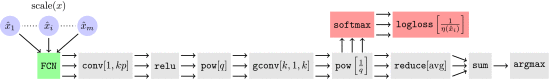
\includegraphics[width=0.95\linewidth]{images/CNNNBNL.png}
\caption{The architecture of the proposed method, fully convolutional CNN-NBNL}
\end{figure}

\subsection{Experimental results}\label{header-n699}

\subsubsection{Proposed method comparison with
baselines}\label{header-n700}

In the first series of experiments, the proposed method is compared with
its non-end-to-end counterpart: a CNN-NBNL approach explained in
{[}18{]}. In addition, other two holistic approaches are chosen for
testing the FC-CNN-NBNL method. Both of them have been proposed by Zhou
\emph{et al.} {[}23{]}, {[}24{]}, in which they pre-train a CNN with a
huge dataset and use it as features extractor for learning a linear SVM
model. To demonstrate the generality of this work, all approaches are
tested through three different base networks: the Caffe {[}20{]} version
of AlexNet {[}19{]}, VGG-16 {[}21{]} and GoogLeNet {[}22{]}. To decide
the proper learning rate schedule and number of epochs, the authors
performed parameters tuning on a separate validation set. As parameters
of the NBNL classifier, the authors chose $k = 10$ and $p = 2$,
applying a weight decay of $10^{-5}$ on the prototypes. Notice that
the model proposed in this work considered 110 descriptors, while 100
were used for the baseline method in {[}13{]}. However, it has been
experimentally verified that a difference of 10 descriptors does not
influence performance. The experiments are performed using three
different datasets: Sports8 (which contains 8 different indoor and
outdoor sport scenes), Scene15 (composed by different categories of
outdoor and indoor scenes) and MIT67 (which contains images of 67 indoor
scenes). For each dataset, the authors took 5 random splits, reporting
the results as mean and standard deviation. The following table shows
the results of this evaluation.

\begin{longtable}[]{@{}lllll@{}}
\toprule
\textbf{Network} & \textbf{Method} & \textbf{Sport8} & \textbf{Scene15}
& \textbf{MIT67}\tabularnewline
\midrule
\endhead
& {[}23{]} & $94.22\pm0.78$ & $91.59\pm0.48$ & 70.8\tabularnewline
AlexNet & {[}18{]} & $95.29 \pm 0.61$ & $92.42 \pm 0.64$ & $73 \pm
0.36$\tabularnewline
& FC-CNN-NBNL & $\boldsymbol{95.58 \pm 0.58}$ & $\boldsymbol{93.63 \pm 0.90}$ &
$\boldsymbol{74.98 \pm 0.78}$\tabularnewline
& {[}24{]} & $91.00$ & 91.25 & 73.30\tabularnewline
GoogLeNet & {[}18{]} & $93.08 \pm 1.78$ & $92.29 \pm 0.59$ & $73.14 \pm
1.43$\tabularnewline
& FC-CNN-NBNL & $\boldsymbol{94.46 \pm 0.86}$ & $\boldsymbol{93.68 \pm 0.57}$ &
$\boldsymbol{80.55 \pm 0.70}$\tabularnewline
& {[}24{]} & 94.17 & 92.12 & 77.63\tabularnewline
VGG-16 & {[}18{]} & $94.79 \pm 0.42$ & $92.97 \pm 0.68$ & $77.62 \pm
0.97$\tabularnewline
& FC-CNN-NBNL & $\boldsymbol{97.04 \pm 0.27}$ & $\boldsymbol{95.12 \pm 0.41}$ &
$\boldsymbol{82.49 \pm 1.35}$\tabularnewline
\bottomrule
\caption{Comparing global and part based CNN models}
\end{longtable}

Mean and standard deviation are provided for FC-CNN-NBNL and {[}13{]}
methods, while for the CNN models in {[}30{]}, {[}31{]} the authors
report results from the original letters. For all base networks and
datasets, the proposed method outperforms the baselines. Moreover, the
end-to-end training model guarantees an improvement in performance
compared to its non-end-to-end counterpart CNN-NBNL. While a pre-trained
CNN isn't able to extract discriminative features when applied to a
specific task, end-to-end training allows to adapting the trained
features to fit a precise task. The figure below shows the difference in
expressivity form feature extracted by {[}18{]} and the proposed method.

\begin{figure}[h!]
\centering
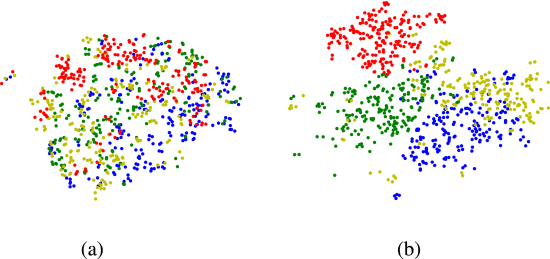
\includegraphics[width=0.8\linewidth]{images/tsneNBNL.png}
\caption{t-SNE visualization of features extracted from 4 classes of the Scene15 dataset: (a) [18], (b) FC-CNN-NBNL}
\end{figure}

To further compare our approach and CNN-NBNL {[}18{]}, the authors also
analyzed the computational time required during the test phase to
process an increasing number of patches. The following figure reports
the results of this analysis: as expected, the fully-convolutional
architecture is greatly advantageous over the CNN-NBNL.

\begin{figure}[h!]
\centering
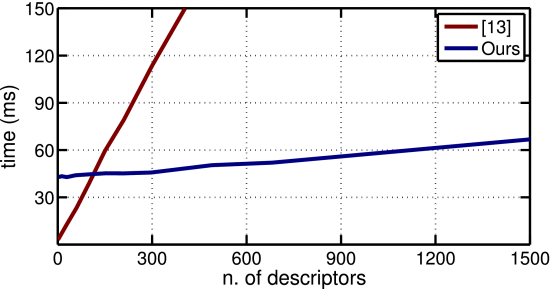
\includegraphics[width=0.7\linewidth]{images/NBNLtime.png}
\caption{Computational time at varying number of descriptors}
\end{figure}

\subsubsection{Proposed method performance in robot place
categorization}\label{header-n767}

These experiments aim to test the proposed method on available robot
datasets, in order to verify its robustness to varying environmental
conditions and occlusions.

The first tested dataset is called \emph{COsy Localization Database}
(COLD). This database contains three datasets of indoor scenes acquired
in three different laboratories from different robots: COLD-Freiburg,
COLD-Ljubljana and COLD-Saarbrucken. These data depict significant
changes with respect to illumination conditions and time of data
acquisition. The models are trained and tested on data collected in the
same laboratory, considering 5 random splits and reporting the average
values. The following table shows the comparison between the CNN
approach explained in {[}23{]} and the proposed method.

\begin{longtable}[]{@{}llll@{}}
\toprule
\textbf{Method} & \textbf{Freiburg} & \textbf{Saarbrcken} &
\textbf{Ljubljana}\tabularnewline
\midrule
\endhead
{[}23{]} & \textbf{96.1} & 96.8 & 98.6\tabularnewline
FC-CNN-NBNL & 95.2 & \textbf{97.3} & \textbf{99.2}\tabularnewline
\bottomrule
\caption{Results on COLD dataset}
\end{longtable}

Despite the {[}23{]} method outperforms the proposed method for
COLD-Freigurg dataset, the high accuracy of our method also demonstrates
that FC-CNN-NBNL is highly effective at discerning among different
rooms, even with significant lighting and environmental changes.

The second dataset used for testing the model proposed is called
\emph{KTH Image Database for rObot Localization} (KTH-IDOL). This
dataset contains image sequences collected by two robots (Dumbo and
Minnie) on 5 different rooms along several days on three different
illumination conditions: sunny, cloudy and night. Using this dataset,
three different types of tests are performed. First, the authors trained
and tested using the same robot and the same weather conditions with one
sequence used for training and another for testing and vice-versa. As a
second experiment, the authors used the same robot for training and
testing, varying the weather conditions of the two sets. In the last
experiment, the classifier is trained with the same weather condition
but it is tested on a different robot. The model proposed in this work
is compared with {[}23{]} and three state-of-the-art approaches:

\begin{itemize}
\item
  {[}25{]} which used high dimensional histogram global features as
  input for a ${\mathcal X}^{2}$ kernel SVM; 
\item
  {[}24{]} which proposed the CENTRIST descriptor and performed nearest
  neighbor classification;
\item
  {[}27{]} which used again the nearest neighbor classifier but with
  Histogram of Oriented Uniform Patterns (HOUP) as features.
\end{itemize}

The following table shows the results of this evaluation (D and M
denotes the names of the robot platform Dumbo and Minnie).

\begin{longtable}[]{@{}llllllll@{}}
\toprule
\textbf{Train} & \textbf{Test} & \textbf{Lighting} & \textbf{{[}25{]}} &
\textbf{{[}26{]}} & \textbf{{[}27{]}} & \textbf{{[}30{]}} &
\textbf{FC-CNN-NBNL}\tabularnewline
\midrule
\endhead
D & D & Same & 97.26 & 97.62 & 98.24 & 97.12 &
\textbf{98.61}\tabularnewline
M & M & Same & 95.51 & 95.35 & 96.61 & 95.19 &
\textbf{97.32}\tabularnewline
D & D & Diff & 80.55 & 94.98 & \textbf{95.76} & 92.33 &
94.17\tabularnewline
M & M & Diff & 71.90 & 90.17 & 92.01 & 88.56 &
\textbf{93.62}\tabularnewline
D & M & Same & 66.63 & 77.78 & 80.05 & 76.22 &
\textbf{87.05}\tabularnewline
M & D & Same & 62.20 & 72.44 & 75.43 & 77.71 &
\textbf{88.51}\tabularnewline
\bottomrule
\caption{Results on KTH-IDOL dataset}
\end{longtable}

The proposed method outperforms all the baselines in the first and third
series of experiments (same lighting). In particular, the large
improvements in performance in the third experiment clearly demonstrates
its ability to generalize over different input representations of the
same scene, independently of the camera mounted on the robot. These
results suggest that it should be possible to train offline our model
and apply it on arbitrary robotic platforms.

\subsection{Conclusions}\label{header-n861}

By seamlessly integrating the CNN and NBNN frameworks, the proposed
approach permits to learn local deep representations, enabling robust
scene recognition. The authors show that their approach outperforms
traditional CNN baselines and previous part-based models that use CNNs
purely as features extractors. In robotics scenarios, the deep network
proposed achieves state-of-the-art results on three different
benchmarks, demonstrating its robustness to occlusions, environmental
changes and different sensors.